%% bare_conf.tex
%% V1.4
%% 2012/12/27
%% by Michael Shell
%% See:
%% http://www.michaelshell.org/
%% for current contact information.
%%
%% This is a skeleton file demonstrating the use of IEEEtran.cls
%% (requires IEEEtran.cls version 1.8 or later) with an IEEE conference paper.
%%
%% Support sites:
%% http://www.michaelshell.org/tex/ieeetran/
%% http://www.ctan.org/tex-archive/macros/latex/contrib/IEEEtran/
%% and
%% http://www.ieee.org/

%%*************************************************************************
%% Legal Notice:
%% This code is offered as-is without any warranty either expressed or
%% implied; without even the implied warranty of MERCHANTABILITY or
%% FITNESS FOR A PARTICULAR PURPOSE!
%% User assumes all risk.
%% In no event shall IEEE or any contributor to this code be liable for
%% any damages or losses, including, but not limited to, incidental,
%% consequential, or any other damages, resulting from the use or misuse
%% of any information contained here.
%%
%% All comments are the opinions of their respective authors and are not
%% necessarily endorsed by the IEEE.
%%
%% This work is distributed under the LaTeX Project Public License (LPPL)
%% ( http://www.latex-project.org/ ) version 1.3, and may be freely used,
%% distributed and modified. A copy of the LPPL, version 1.3, is included
%% in the base LaTeX documentation of all distributions of LaTeX released
%% 2003/12/01 or later.
%% Retain all contribution notices and credits.
%% ** Modified files should be clearly indicated as such, including  **
%% ** renaming them and changing author support contact information. **
%%
%% File list of work: IEEEtran.cls, IEEEtran_HOWTO.pdf, bare_adv.tex,
%%                    bare_conf.tex, bare_jrnl.tex, bare_jrnl_compsoc.tex,
%%                    bare_jrnl_transmag.tex
%%*************************************************************************

% *** Authors should verify (and, if needed, correct) their LaTeX system  ***
% *** with the testflow diagnostic prior to trusting their LaTeX platform ***
% *** with production work. IEEE's font choices can trigger bugs that do  ***
% *** not appear when using other class files.                            ***
% The testflow support page is at:
% http://www.michaelshell.org/tex/testflow/



% Note that the a4paper option is mainly intended so that authors in
% countries using A4 can easily print to A4 and see how their papers will
% look in print - the typesetting of the document will not typically be
% affected with changes in paper size (but the bottom and side margins will).
% Use the testflow package mentioned above to verify correct handling of
% both paper sizes by the user's LaTeX system.
%
% Also note that the "draftcls" or "draftclsnofoot", not "draft", option
% should be used if it is desired that the figures are to be displayed in
% draft mode.
%
\documentclass[conference]{IEEEtran}
\usepackage[utf8]{inputenc}
\usepackage{amsthm}
\newtheorem{mydef}{Definición}

\usepackage[T1]{fontenc}

% Add the compsoc option for Computer Society conferences.
%
% If IEEEtran.cls has not been installed into the LaTeX system files,
% manually specify the path to it like:
% \documentclass[conference]{../sty/IEEEtran}





% Some very useful LaTeX packages include:
% (uncomment the ones you want to load)


% *** MISC UTILITY PACKAGES ***
%
%\usepackage{ifpdf}
% Heiko Oberdiek's ifpdf.sty is very useful if you need conditional
% compilation based on whether the output is pdf or dvi.
% usage:
% \ifpdf
%   % pdf code
% \else
%   % dvi code
% \fi
% The latest version of ifpdf.sty can be obtained from:
% http://www.ctan.org/tex-archive/macros/latex/contrib/oberdiek/
% Also, note that IEEEtran.cls V1.7 and later provides a builtin
% \ifCLASSINFOpdf conditional that works the same way.
% When switching from latex to pdflatex and vice-versa, the compiler may
% have to be run twice to clear warning/error messages.






% *** CITATION PACKAGES ***
%
%\usepackage{cite}
% cite.sty was written by Donald Arseneau
% V1.6 and later of IEEEtran pre-defines the format of the cite.sty package
% \cite{} output to follow that of IEEE. Loading the cite package will
% result in citation numbers being automatically sorted and properly
% "compressed/ranged". e.g., [1], [9], [2], [7], [5], [6] without using
% cite.sty will become [1], [2], [5]--[7], [9] using cite.sty. cite.sty's
% \cite will automatically add leading space, if needed. Use cite.sty's
% noadjust option (cite.sty V3.8 and later) if you want to turn this off
% such as if a citation ever needs to be enclosed in parenthesis.
% cite.sty is already installed on most LaTeX systems. Be sure and use
% version 4.0 (2003-05-27) and later if using hyperref.sty. cite.sty does
% not currently provide for hyperlinked citations.
% The latest version can be obtained at:
% http://www.ctan.org/tex-archive/macros/latex/contrib/cite/
% The documentation is contained in the cite.sty file itself.






% *** GRAPHICS RELATED PACKAGES ***
%
\usepackage[lofdepth,lotdepth]{subfig}
\usepackage{graphicx}
\usepackage{caption}
% \usepackage{subcaption}
% \else
%   % or other class option (dvipsone, dvipdf, if not using dvips). graphicx
%   % will default to the driver specified in the system graphics.cfg if no
%   % driver is specified.
%   % \usepackage[dvips]{graphicx}
%   % declare the path(s) where your graphic files are
%   % \graphicspath{{../eps/}}
%   % and their extensions so you won't have to specify these with
%   % every instance of \includegraphics
%   % \DeclareGraphicsExtensions{.eps}
% \fi
% graphicx was written by David Carlisle and Sebastian Rahtz. It is
% required if you want graphics, photos, etc. graphicx.sty is already
% installed on most LaTeX systems. The latest version and documentation
% can be obtained at:
% http://www.ctan.org/tex-archive/macros/latex/required/graphics/
% Another good source of documentation is "Using Imported Graphics in
% LaTeX2e" by Keith Reckdahl which can be found at:
% http://www.ctan.org/tex-archive/info/epslatex/
%
% latex, and pdflatex in dvi mode, support graphics in encapsulated
% postscript (.eps) format. pdflatex in pdf mode supports graphics
% in .pdf, .jpeg, .png and .mps (metapost) formats. Users should ensure
% that all non-photo figures use a vector format (.eps, .pdf, .mps) and
% not a bitmapped formats (.jpeg, .png). IEEE frowns on bitmapped formats
% which can result in "jaggedy"/blurry rendering of lines and letters as
% well as large increases in file sizes.
%
% You can find documentation about the pdfTeX application at:
% http://www.tug.org/applications/pdftex





% *** MATH PACKAGES ***
%
%\usepackage[cmex10]{amsmath}
% A popular package from the American Mathematical Society that provides
% many useful and powerful commands for dealing with mathematics. If using
% it, be sure to load this package with the cmex10 option to ensure that
% only type 1 fonts will utilized at all point sizes. Without this option,
% it is possible that some math symbols, particularly those within
% footnotes, will be rendered in bitmap form which will result in a
% document that can not be IEEE Xplore compliant!
%
% Also, note that the amsmath package sets \interdisplaylinepenalty to 10000
% thus preventing page breaks from occurring within multiline equations. Use:
%\interdisplaylinepenalty=2500
% after loading amsmath to restore such page breaks as IEEEtran.cls normally
% does. amsmath.sty is already installed on most LaTeX systems. The latest
% version and documentation can be obtained at:
% http://www.ctan.org/tex-archive/macros/latex/required/amslatex/math/





% *** SPECIALIZED LIST PACKAGES ***
%
%\usepackage{algorithmic}
% algorithmic.sty was written by Peter Williams and Rogerio Brito.
% This package provides an algorithmic environment fo describing algorithms.
% You can use the algorithmic environment in-text or within a figure
% environment to provide for a floating algorithm. Do NOT use the algorithm
% floating environment provided by algorithm.sty (by the same authors) or
% algorithm2e.sty (by Christophe Fiorio) as IEEE does not use dedicated
% algorithm float types and packages that provide these will not provide
% correct IEEE style captions. The latest version and documentation of
% algorithmic.sty can be obtained at:
% http://www.ctan.org/tex-archive/macros/latex/contrib/algorithms/
% There is also a support site at:
% http://algorithms.berlios.de/index.html
% Also of interest may be the (relatively newer and more customizable)
% algorithmicx.sty package by Szasz Janos:
% http://www.ctan.org/tex-archive/macros/latex/contrib/algorithmicx/




% *** ALIGNMENT PACKAGES ***
%
%\usepackage{array}
% Frank Mittelbach's and David Carlisle's array.sty patches and improves
% the standard LaTeX2e array and tabular environments to provide better
% appearance and additional user controls. As the default LaTeX2e table
% generation code is lacking to the point of almost being broken with
% respect to the quality of the end results, all users are strongly
% advised to use an enhanced (at the very least that provided by array.sty)
% set of table tools. array.sty is already installed on most systems. The
% latest version and documentation can be obtained at:
% http://www.ctan.org/tex-archive/macros/latex/required/tools/


% IEEEtran contains the IEEEeqnarray family of commands that can be used to
% generate multiline equations as well as matrices, tables, etc., of high
% quality.




% *** SUBFIGURE PACKAGES ***
%\ifCLASSOPTIONcompsoc
%  \usepackage[caption=false,font=normalsize,labelfont=sf,textfont=sf]{subfig}
%\else
%  \usepackage[caption=false,font=footnotesize]{subfig}
%\fi
% subfig.sty, written by Steven Douglas Cochran, is the modern replacement
% for subfigure.sty, the latter of which is no longer maintained and is
% incompatible with some LaTeX packages including fixltx2e. However,
% subfig.sty requires and automatically loads Axel Sommerfeldt's caption.sty
% which will override IEEEtran.cls' handling of captions and this will result
% in non-IEEE style figure/table captions. To prevent this problem, be sure
% and invoke subfig.sty's "caption=false" package option (available since
% subfig.sty version 1.3, 2005/06/28) as this is will preserve IEEEtran.cls
% handling of captions.
% Note that the Computer Society format requires a larger sans serif font
% than the serif footnote size font used in traditional IEEE formatting
% and thus the need to invoke different subfig.sty package options depending
% on whether compsoc mode has been enabled.
%
% The latest version and documentation of subfig.sty can be obtained at:
% http://www.ctan.org/tex-archive/macros/latex/contrib/subfig/




% *** FLOAT PACKAGES ***
%
%\usepackage{fixltx2e}
% fixltx2e, the successor to the earlier fix2col.sty, was written by
% Frank Mittelbach and David Carlisle. This package corrects a few problems
% in the LaTeX2e kernel, the most notable of which is that in current
% LaTeX2e releases, the ordering of single and double column floats is not
% guaranteed to be preserved. Thus, an unpatched LaTeX2e can allow a
% single column figure to be placed prior to an earlier double column
% figure. The latest version and documentation can be found at:
% http://www.ctan.org/tex-archive/macros/latex/base/


%\usepackage{stfloats}
% stfloats.sty was written by Sigitas Tolusis. This package gives LaTeX2e
% the ability to do double column floats at the bottom of the page as well
% as the top. (e.g., "\begin{figure*}[!b]" is not normally possible in
% LaTeX2e). It also provides a command:
%\fnbelowfloat
% to enable the placement of footnotes below bottom floats (the standard
% LaTeX2e kernel puts them above bottom floats). This is an invasive package
% which rewrites many portions of the LaTeX2e float routines. It may not work
% with other packages that modify the LaTeX2e float routines. The latest
% version and documentation can be obtained at:
% http://www.ctan.org/tex-archive/macros/latex/contrib/sttools/
% Do not use the stfloats baselinefloat ability as IEEE does not allow
% \baselineskip to stretch. Authors submitting work to the IEEE should note
% that IEEE rarely uses double column equations and that authors should try
% to avoid such use. Do not be tempted to use the cuted.sty or midfloat.sty
% packages (also by Sigitas Tolusis) as IEEE does not format its papers in
% such ways.
% Do not attempt to use stfloats with fixltx2e as they are incompatible.
% Instead, use Morten Hogholm'a dblfloatfix which combines the features
% of both fixltx2e and stfloats:
%
% \usepackage{dblfloatfix}
% The latest version can be found at:
% http://www.ctan.org/tex-archive/macros/latex/contrib/dblfloatfix/




% *** PDF, URL AND HYPERLINK PACKAGES ***
%
%\usepackage{url}
% url.sty was written by Donald Arseneau. It provides better support for
% handling and breaking URLs. url.sty is already installed on most LaTeX
% systems. The latest version and documentation can be obtained at:
% http://www.ctan.org/tex-archive/macros/latex/contrib/url/
% Basically, \url{my_url_here}.




% *** Do not adjust lengths that control margins, column widths, etc. ***
% *** Do not use packages that alter fonts (such as pslatex).         ***
% There should be no need to do such things with IEEEtran.cls V1.6 and later.
% (Unless specifically asked to do so by the journal or conference you plan
% to submit to, of course. )


% correct bad hyphenation here
\hyphenation{op-tical net-works semi-conduc-tor}


\begin{document}
%
% paper title
% can use linebreaks \\ within to get better formatting as desired
% Do not put math or special symbols in the title.
\title{Problema del Clique Máximo: Estrategias altamente paralelizables}


% author names and affiliations
% use a multiple column layout for up to three different
% affiliations
\author{\IEEEauthorblockN{Simón Castillo}
\IEEEauthorblockA{Departamento de Computación y\\Tecnología de la Información\\
Universidad Simón Bolívar\\
Sartenejas, Caracas, Venezuela\\
Email: simoncastillo@gmail.com}
\and
\IEEEauthorblockN{Alejandro Flores}
\IEEEauthorblockA{
Departamento de Computación y\\Tecnología de la Información\\
Universidad Simón Bolívar\\
Sartenejas, Caracas, Venezuela\\
Email: alejandroflores.af@gmail.com
}}

% conference papers do not typically use \thanks and this command
% is locked out in conference mode. If really needed, such as for
% the acknowledgment of grants, issue a \IEEEoverridecommandlockouts
% after \documentclass

% for over three affiliations, or if they all won't fit within the width
% of the page, use this alternative format:
%
%\author{\IEEEauthorblockN{Michael Shell\IEEEauthorrefmark{1},
%Homer Simpson\IEEEauthorrefmark{2},
%James Kirk\IEEEauthorrefmark{3},
%Montgomery Scott\IEEEauthorrefmark{3} and
%Eldon Tyrell\IEEEauthorrefmark{4}}
%\IEEEauthorblockA{\IEEEauthorrefmark{1}School of Electrical and Computer Engineering\\
%Georgia Institute of Technology,
%Atlanta, Georgia 30332--0250\\ Email: see http://www.michaelshell.org/contact.html}
%\IEEEauthorblockA{\IEEEauthorrefmark{2}Twentieth Century Fox, Springfield, USA\\
%Email: homer@thesimpsons.com}
%\IEEEauthorblockA{\IEEEauthorrefmark{3}Starfleet Academy, San Francisco, California 96678-2391\\
%Telephone: (800) 555--1212, Fax: (888) 555--1212}
%\IEEEauthorblockA{\IEEEauthorrefmark{4}Tyrell Inc., 123 Replicant Street, Los Angeles, California 90210--4321}}




% use for special paper notices
%\IEEEspecialpapernotice{(Invited Paper)}




% make the title area
\maketitle

% As a general rule, do not put math, special symbols or citations
% in the abstract
% \begin{abstract}
% The abstract goes here.
% \end{abstract}

% no keywords




% For peer review papers, you can put extra information on the cover
% page as needed:
% \ifCLASSOPTIONpeerreview
% \begin{center} \bfseries EDICS Category: 3-BBND \end{center}
% \fi
%
% For peerreview papers, this IEEEtran command inserts a page break and
% creates the second title. It will be ignored for other modes.
\IEEEpeerreviewmaketitle



\section{Introducción}
\label{sec:intro}

El problema del \textsf{MAXCLIQUE} (abreviado MCP por sus siglas en
inglés) es un problema clásico de optimización combinatoria, el cual
posee importantes aplicaciones en diferentes dominios como teoría de
códigos, diagnóstico de fallas o visión por computadoras. De manera
informal, el problema consiste en encontrar un subgrafo completo de
tamaño máximo. En general, este problema es inmanejable, por lo que se
ha invertido una cantidad de tiempo y esfuerzo en lograr diseñar
algoritmos que generen soluciones óptimas de este problema en un
tiempo razonable.

Durante los últimos años, la utilización de cliques como parte
fundamental para determinar la estructura de diversos problemas ha ido
considerablemente en aumento. Dichos problemas residen en las áreas de
las ciencias sociales, biológicas, financieras, entre otras; donde
cada uno de ellos dependen de la búsqueda de cliques en redes de gran
densidad. Esto convierte al problema computacionalmente costoso, tanto
para realizar el cálculo, como para ser representado por un computador
(i.e. los grafos originales no pueden ser cargados en memoria
principal, por lo que muchas veces es necesario guardar la estructura
del grafo en memoria secundaria e ir cargando a medida que se vaya
necesitando).

La literatura cuenta con gran cantidad de aportes que intentan
resolver este importante problema de la teoría de grafos. En
particular, diversas técnicas meta-heurísticas se han aplicado para
tratar de conseguir cliques máximos en un tiempo de computo
razonable. En particular, el estado del arte se ha enfocado en el uso
de técnicas basadas en la búsqueda local como lo son la búsqueda tabú,
la búsqueda $k$-opt, vecindades variables, entre otras. Asímismo, las
técnicas meta-heurísticas basadas en población han recibido
considerables contribuciones, en particular los algoritmos genéticos,
para la cual el problema en principio se presta muy bien, y, en menor
medida, la optimización por colonias de hormigas.

A partir de finales de la década pasada, los procesadores multi-núcleo
se han vuelto altamente disponible en el mercado de consumidores. Este
hecho presenta nuevas posibilidades para problemas computacionales
altamente costosos donde se podría conseguir más y mejores resultados
de ser posible paralelizar la carga de computo en múltiples instancias
que realicen la búsqueda de soluciones en paralelo para luego
consolidarlas en una mejor solución. Para el conocimiento de los
autores, para el problema no se ha intentado paralelizar con éxito. El
principal aporte que presentaremos en el presente trabajo es un
estudio de dos técnicas de búsqueda meta-heurística que resultan
comportarse sumamente bien al ser paralelizadas en múltiples
núcleos. En primera instancia, consideraremos la técnica presentada
por \cite{dynamicl}, conocida como \emph{Dynamic Local Search} (DLS), considerada
una técnica del estado del arte para la búsqueda de
cliques. Posteriormente, consideraremos la optimización por colonia de
hormigas, basados en el trabajo por \cite{aco1, aco2}, la cuál
expandiremos utilizando búsqueda local aprovechando DLS.

% Como un breve ejemplo tenemos la industria farmacéutica y agroquímica,
% en las cuales establecer relaciones estructurales entre pares de
% estructuras moleculares de tres dimensiones es un problema
% importante. Estas estructuras moleculares de tres dimensiones pueden
% ser representadas usando grafos. Para cada pareja de moléculas un
% subgrafo completo común máximo, hace referencia a la mayor cantidad de
% átomos que tienen la misma distancia entre átomos. Por lo que este
% tipo de subgrafos, provee una métrica sencilla para medir la similitud
% estructural y provee información sobre ambas moléculas. Éste es sólo
% un ejemplo concreto de las numerosas posibles aplicaciones de
% \textsf{MAXCLIQUE}. Además, es evidente que aplicaciones de este
% problema surgen siempre que se consideran múltiples estructuras que
% pueden estar relacionadas entre sí (por ejemplo, redes sociales,
% mineria de datos, entre otras). \cite{survey-clique} realiza un
% recorrido de algunos de los retos puntuales que se deben superar en el
% problema de la búsqueda de cliques en grafos de gran tamaño, junto con
% aplicaciones concretas de los mismos.

El presente trabajo está organizado como sigue: en la sección
\ref{sec:prev-work} presentamos un breve análisis de diferentes
métodos encontrados en la literatura disponible, en la sección
\ref{sec:defs} presentamos un resumen general de la notación y
conceptos básicos que utilizaremos, en la sección \ref{sec:dls}
presentamos la descripción de DLS junto al proceso empleado para
volver el algoritmo paralelo, \ref{sec:aco} presentamos el marco de
trabajo para la optimización por medio de colonias de hormiga y de
igual forma su proceso de paralelización, en las \ref{sec:experiments}
presentamos la evaluación experimental de las técnicas empleadas y
finalmente en la sección \ref{sec:conclusions} presentamos
conclusiones y direcciones futuras.

\section{Trabajo Previo}
\label{sec:prev-work}

\textsf{MAXCLIQUE} es unos de los problemas originales de Karp
\cite{karp} que fueron demostrados como \textsc{NP}-completo, es
decir, a menos que \textsc{P} = \textsc{NP}, algoritmos exactos están
garantizados a devolver una solución sólo en un tiempo que incrementa
exponencialmente con el número de nodos en el grafo. Más aún,
\cite{arora1} probó que para algún $\epsilon > 0$ la aproximación del
número de clique dentro de un factor de $|V|^\epsilon$ es
\textsc{NP}-duro; de hecho, el mejor algoritmo aproximado en tiempo
polinomial requiere $O(|V|/(\log{|V|})^2)$ \cite{best-approx}.

Aunque clásicamente \textsf{MAXCLIQUE} es encontrado en la literatura
como su variante en forma de problema de decisión
\textsc{NP}-completo, el problema de optimización se presta a diversas
técnicas de optimización combinatoria. Desde un punto de vista
práctico, algoritmos exactos son capaces de dar respuesta con
instancias de grafos en el orden de los cientos de nodos
\cite{oster,shinano, wood}. Sin embargo, para poder manejar instancias
mucho más complejas (i.e. grafos con una cardinalidad de órdenes de
magnitud mayores), diversas técnicas del estado del arte emplean
diversas metaheurísticas.  De igual forma, es importante destacar que
el problema de \textsf{MAXCLIQUE} es polinomialmente equivalente a
\textsf{INDEPENDENTSET} así como al \textsf{MINVERTEXCOVER}, por lo
que cualquier heurística que funcione para estos problemas dará buenos
resultados para el problema \textsf{MAXCLIQUE} \cite{Bomze99}.

A pesar del considerable esfuerzo que se ha volcado en el desarrollo
de métodos basados en heurísticas, no existe un solo método que
obtenga los mejores resultados. De hecho, a pesar de la dificultad que
puede existir en comparar diversos métodos (i.e. diferencias en donde
se corren las pruebas), es posible diferenciar varios métodos que
podemos considerar estado del arte: \emph{Reactive Local Search}
\cite{rls}, un método basado en búsqueda tabú que adapta
automaticamente el parámetro de tenencia de la tabla tabú, \emph{Deep
  Adaptive Greedy Search} \cite{grosso}, la cuál utiliza un algoritmo
voraz iterativo, \emph{búsqueda k-opt} \cite{kopt}, basado en
\emph{Variable Depth Search} aumentado con una heurística simple de
agregación o remoción de vértices del mejor clique conseguido hasta el
momento, \emph{VNS} \cite{vns}, basado en \emph{vecindades
  variables} con búsqueda voraz en la vecindades, y \emph{Dynamic
  Local Search-Maximum Clique} \cite{dynamicl}, una heurística que
alterna fases de mejoramiento iterativo (donde los vértices son
agregados al clique), con búsqueda en los \emph{plateau} (donde
vértices agregados al clique son cambiados por vértices que no se
encuentran en el clique).

Las técnicas basadas en búsqueda local toman un lugar importante en
este problema. En particular, como podemos ver en \cite{old1, old2,
  multistart}, la búsqueda tabú resulta ser un método no solo muy
estudiado sino sino que arroja resultados prometedores. En particular,
\cite{old1, old2}, de los primeros en estudiar la búsqueda tabú para
el problema del clique máximo, implementan dos variantes de la
búsqueda tabú: una que funciona de forma determinista y una que
funciona de forma probabilista. En estos métodos se varía
considerablemente los parametros de tenencia y se estudia su efecto
sobre el problema. Sin embargo, resulta interesante para nuestros
intereses estudiar la búsqueda $k$-opt presentada en \cite{kopt}. Esta
simple heurística consiste en la en una búsqueda basada en vecindarios
variables donde se alternan las fases de intensificación (agregar
vértices al clique) con fases de eliminación de vértices cuya remoción
permita agregar nuevos vértices posteriormente. Esta simple
heurística, cuyo proceso de selección de vértices esta basado no más
que en el grado de los vértices, resulta ser sumamente efectiva para
el problema del clique máximo. De esta forma, no solo son capaces de
dar resultados que son considerados del estado del arte, sino que es
capaz de hacerlo en un tiempo de ejecución muy rápido.

A partir de las ideas implementadas en la búsqueda $k$-opt se derivan
dos heurísticas muy similares: \emph{Deep Adaptive Greedy Search}
(DAGS) y \emph{Dynamic Local Search} (DLS). Estas dos heurísticas, de
igual forma, alternan fases de intensificación de la búsqueda con
remoción de vértices (búsqueda \emph{plateau}). Sin embargo, agregan
un mecanismo numérico de diversificación de la búsqueda que los
autores de DLS en \cite{dynamicl} llaman \emph{tabla de
  penalización}. Esta tabla, asigna a cada vértice una penalización al
final de cada ciclo de búsqueda, donde los vértices asociados a un
clique aumentan su valor de penalización, y designa que el criterio de
selección de cada vértice sea el vértice con el mínimo valor de
penalización disponible. Este criterio no solo permite diversificar
considerablemente la búsqueda sino que permite disminuir
considerablemente los estados (cliques) previamente visitados y
permite visitar rápidamente el espacio de búsqueda.

De igual forma, los algoritmos basados en el funcionamiento de la
naturaleza son capaces de conseguir buenos resultados al problema. En
particular, la investigación de métodos basados en algoritmos
genéticos constituye una parte considerable de la literatura asociada
al problema del \textsf{MAXCLIQUE}. En \cite{hybgen} se presenta una
nueva técnica híbrida basada en algoritmos genéticos y se realiza una
comparación de varios algoritmos evolutivos. Sin embargo, a pesar de
ser capaz de dar mejores resultados que los otros algoritmos
evolutivos, el método presentado no supera los resultados obtenidos
con métodos no evolutivos. Por otra parte, los cliques son utilizados
considerablemente para estudiar la estructura interna de las moléculas
en las ciencias biológicas y la química orgánica, por lo que diversos
métodos de búsqueda de cliques en espacios tridimensionales han sido
estudiados \cite{mce,protein}. Otro método basado en observaciones de
la naturaleza, aunque mucho menos estudiado que los algoritmos
genéticos, que ha resultado en buenos resultados con respecto al
estado del arte constituye la optimización por colonias de hormigas
(\emph{ant colony optimization}, ACO).

Aunque no tan influyentes como otros trabajos en la literatura del
clique máximo, en \cite{aco1, aco2} se estudian las capacidades de ACO
en dos instanciaciones genéricas del problema las cuales generan
cliques maximales sucesivos y utilizando una heurística voráz para
seleccionar cada vértice nuevo a ser agregado. Posteriormente, estos
cliques conseguidos son mejorados por búsqueda local basada en un
criterio de selección muy parecido al utilizado en GRASP y similar al
usado en DLS. Los resultados obtenidos muestran que ACO es competitivo
con otros métodos heurísticos del estado del arte, y que al agregar
búsqueda local el tiempo de corrida mejora considerablemente. Además,
en estos trabajos no solo se realiza un estudio de la calidad de las
soluciones sino como el problema del clique máximo se presta para ser
explotado por ACO. Asimismo, en estos trabajos, como resultado
importante se presentan dos heurísticas para la asignación de las
feromonas que las hormigas siguen: \texttt{Vertex-AC} y
\texttt{Edge-AC}. La primera, considera colocar las feromonas sobre
cada vértice mientras que la segunda considera colocar las feromonas
sobre cada lado. Para nuestros intereses, únicamente consideraremos la
primera heurística, \texttt{Verte-AC} la cual trataremos de expandir
con el uso de DLS.

\section{Definiciones}
\label{sec:defs}

Usaremos la siguiente notación: $G = (V,E)$ denota un grafo no
dirigido donde, sin perder generalidad, $V = \{1, 2, 3, …, n\}$ y $E
\subseteq \{(i, j): i, j \in V\}$. $N(i)$ con $i \in V$ representa la
vecindad del vértice $i$ (i.e. los vertices adyacentes a $i$).

\begin{mydef}
  Dado un grafo no dirigido $G = (V,E)$, donde $V$ es el conjunto
  de vértices y $E \subseteq V \times V$ el conjunto de lados, un
  \textbf{clique} es un conjunto de vértices $C \subseteq V$ tal que cada
  pareja de vértices distintos de $C$ está conectado por un lado en
  $E$, es decir, el subgrafo inducido por $C$ es completo.
\end{mydef}

\begin{mydef}
  Un \emph{clique} es \textbf{parcial} si está estrictamente incluído
  en otro (es decir, su cardinalidad puede aumentarse añadiendo
  vértices pertenecientes a $E$ a dicho clique); de lo contrario es
  \textbf{maximal}.
\end{mydef}

\begin{mydef}
  Un \textbf{clique máximo} es un clique maximal de cardinalidad máxima.
\end{mydef}

En la Fig. \ref{fig_sim} se encuentran ejemplos de estas definiciones
para un grafo $G_1$. Claramente, podemos observar que todo clique
máximo es necesariamente máximal por definición, pero todo clique
máximal no necesariamente es máximo. El problema de enumerar los
cliques maximales de un grafo ha recibido considerable atención en la
literatura, en particular el algoritmo de Bron-Kerbosch
\cite{Bron:1973:AFC:362342.362367} es capaz de enumerar todos los
cliques maximales de un grafo utilizando búsqueda recursiva. De esta
forma, es posible conseguir un algoritmo ingenuo para el problema del
clique máximo, el cual funciona enumerando todos los cliques de un
grafo y tomando el de máxima cardinalidad. Todas las técnicas
meta-heurísticas que estudiaremos parten de la noción de conseguir
cliques maximales y mejorarlos de diversas maneras.

\begin{mydef}
  Dado un grafo $G = (V, E)$, la cardinalidad del clique máximo se
  denota $\omega(G)$. Este valor se conoce como el número de clique.
\end{mydef}

\begin{mydef}
  Dado un grafo $G = (V,E)$ arbitrario, decidir si $G$ tiene un clique
  de tamaño $k$ es un problema \textsc{NP}-completo.
\end{mydef}

\begin{mydef}
  Dado un grafo $G = (V,E)$ arbitrario, conseguir un clique máximo en
  el grafo $G$, es decir, conseguir un subgrafo completo $G’$ de
  cardinalidad máxima es \textsc{NP}-duro.
\end{mydef}

\begin{figure*}[!t]
\centering
\subfloat[Grafo $G_1$ con su clique máximo resaltado en rojo]{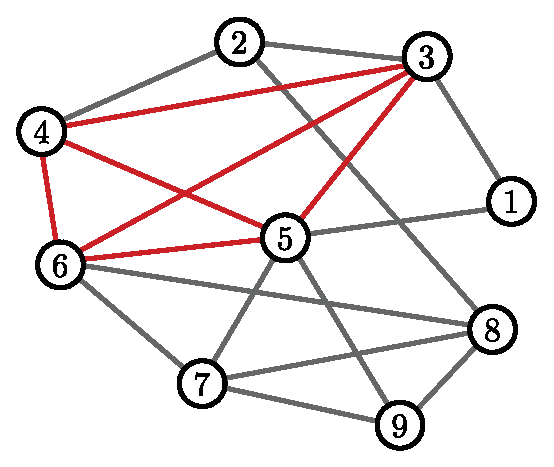
\includegraphics[width=3.5in]{Grafo}%
\label{fig_first_case}}
\hfil
\subfloat[Clique máximal y parcial del grafo $G_1$]{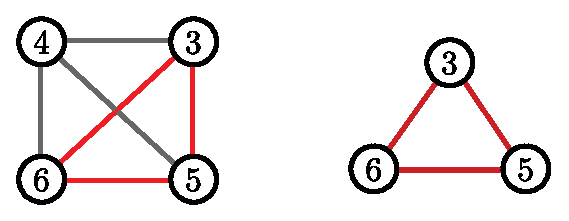
\includegraphics[width=3.5in]{Cliques}%
\label{fig_second_case}}
\caption{Diversos cliques según las definiciones expuestas en el grafo
$G_1$ formado por 9 vértices y 18 lados. }
\label{fig_sim}
\end{figure*}


En este trabajo nos dedicaremos a estudiar el problema de
optimización, es decir, el problema de conseguir un clique de tamaño
máximo.

\begin{mydef}
  Dado un grafo $G = (V,E)$ arbitrario y un clique $C$ en este grafo,
  llamamos a su \textbf{conjunto de mejoramiento} al conjunto de $I
  \subseteq V$ tal que para $x \in I$ se tiene que $x$ está conectado a
  todos los elementos de $C$ en $G$.
\end{mydef}


El conjunto de mejoramiento también se conoce como el conjunto de
candidatos. Un clique máximal claramente tiene un conjunto de
mejoramiento vacío.

\begin{mydef}
  Dado un grafo $G = (V,E)$ arbitrario y un clique $C$ en este grafo,
  llamamos a su \textbf{conjunto de nivel} al conjunto $L \subseteq V$
  tal que para $x \in L$ se tiene que $x$ esta conectado a todos los
  elementos de $C$ en $G$ menos \emph{exactamente} uno. Para cada
  elemento $x \in L$, el elemento $y \in C$ tal que no existe $(x,y)
  \in E$ se le conoce como el \textbf{dual} de $x$.
\end{mydef}

El conjunto de nivel de un clique $C$ en un grafo $G$ permite realizar
intercambio elemento a elemento por su dual. Este proceso resulta ser
la base para el proceso de búsqueda por fases de los diversos
algoritmos que combinan métodos de intensificación con remoción de
vértices.

\section{Búsqueda Dinámica Local}
\label{sec:dls}

\section{Optimización por Colonia de Hormigas}
\label{sec:aco}

\section{Experimentos y resultados}
\label{sec:experiments}

\section{Conclusiones y futuras direcciones}
\label{sec:conclusions}




% \begin{thebibliography}{1}

% % \bibitem{IEEEhowto:kopka}
% % H.~Kopka and P.~W. Daly, \emph{A Guide to \LaTeX}, 3rd~ed.\hskip 1em plus
% %   0.5em minus 0.4em\relax Harlow, England: Addison-Wesley, 1999.

% \end{thebibliography}
\bibliographystyle{plain}
\bibliography{biblio}



% that's all folks
\end{document}
